% !TEX encoding = UTF-8
% !TEX TS-program = pdflatex
% !TEX root = ../tesi.tex

%**************************************************************
\chapter{\textit{License Manager 1.0}}
\label{cap:license-manager}
%**************************************************************

\textit{License Manager 1.0} nasce con lo scopo di creare nuove licenze, eliminando \textit{GenPK} e le problematiche ad esso correlate. Nel corso dello stage, con il delinearsi di nuovi obiettivi, il programma è stato ampliato per poter gestire la maggior parte degli aspetti di una licenza, incluso il monitoraggio. Le funzionalità del Software sono svolte tramite chiamate a Web Service, i quali utilizzano il Database \texttt{DBLicenze} per il salvataggio dei dati.
\\
Inizialmente pensato per un uso interno all'azienda, grazie alle molteplici funzionalità che esso offriva, è stato deciso di distribuire il Software anche ai rivenditori, concedendo loro una maggior capacità operativa.
I rivenditori, per la sicurezza dell'azienda, possono usufruire di operazioni limitate, e le modifiche più rilevanti sono comunicate a \textit{VISIONEIMPRESA s.r.l.} tramite mail.


%**************************************************************
\section{Scopo del prodotto}

Con \textit{License Manager 1.0} si vuole racchiudere in un unico programma la gestione completa delle licenze del \textit{Software Gestionale Vision}, dalla creazione all'eliminazione, con la possibilità di effettuare modifiche, ricevere statistiche e monitorare lo stato delle licenze per notare possibili anomalie. 

%**************************************************************

\section{Tipologie di utenti}

\textit{License Manager 1.0} gestisce due tipologie di utente, \textit{Admin} e \textit{Guest}.

\begin{itemize}
\item \textbf{\textit{Admin}}: ha a disposizione tutte le funzionalità senza limitazioni, ed è ideato per i soli membri dell’azienda. Un utente di questo tipo può visualizzare e modificare tutte le licenze, indipendentemente da chi le abbia create;

\item \textbf{\textit{Guest}}: ha a disposizione tutte le funzionalità ma con alcune limitazioni. Questo tipo di utente è creato per ogni rivenditore, in modo che esso possa gestire solo le licenze da esso vendute, senza interferire con le licenze create dall’azienda o da altri rivenditori. Ad ogni \textit{Guest} è associato un \texttt{Codice Utente}, ossia un codice definito per lo specifico rivenditore, e più \textit{Guest} possono avere lo stesso \texttt{Codice Utente}, poiché un rivenditore potrebbe voler affidare la gestione delle proprie licenze ad utenti diversi.
\end{itemize}


%**************************************************************
\section{Autenticazione}
Poiché il programma si propone di gestire diverse tipologie di utenti è stato implementato un sistema di autenticazione. In Figura \ref{auth} è mostrato il Form di autenticazione, visibile all'avvio del programma.

\begin{figure}[!h] 
    \centering 
    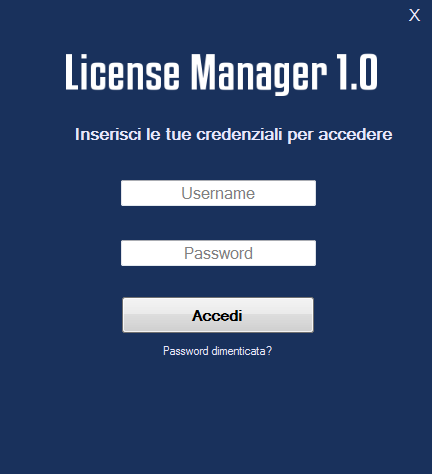
\includegraphics[width=0.5\columnwidth]{LicenseManager/auth} 
    \caption{License Manager 1.0 - Form di autenticazione.}
    \label{auth}
\end{figure}

L’utente, per accedere, deve inserire il proprio \texttt{Username} e la \texttt{Password}, e cliccare su "Accedi".\\
Solo gli \textit{Admin} possono creare gli utenti, scegliendone l’username, un indirizzo email da associare, e nel caso l’utente sia destinato a un rivenditore è data la possibilità di sceglierne il \texttt{Codice Utente} (o codice rivenditore).
Un utente che ha dimenticato la password è costretto a contattare un \textit{Admin} per chiederne il reset. Se l’\textit{Admin} concede il reset della password, inserendo l’\texttt{Username} e cliccando su "Password dimenticata?" è possibile impostare una nuova Password.\\
Per maggiori dettagli sulla gestione degli utenti si rimanda alla sezione \ref{ammut}.
\newpage


%**************************************************************
\section{Struttura generale del Software}
Dopo l'autenticazione, il programma si mostra come in Figura \ref{primscher}.

\begin{figure}[!h] 
    \centering 
    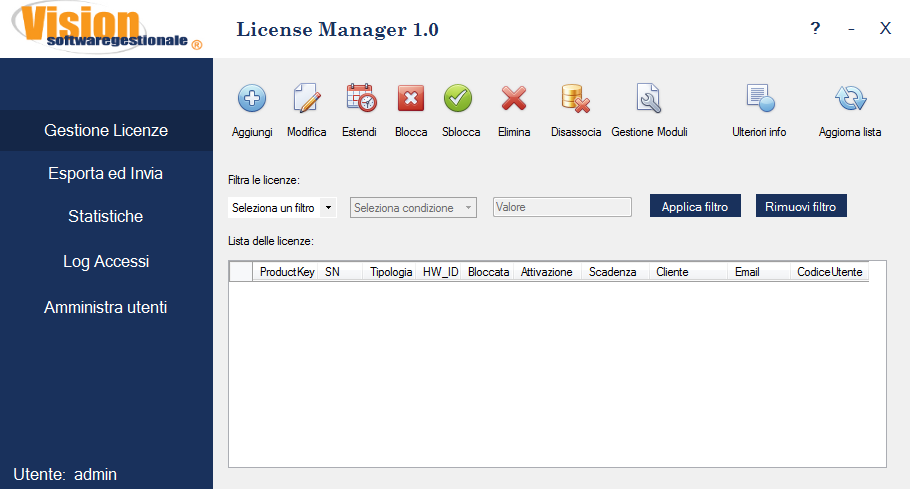
\includegraphics[width=1\columnwidth]{LicenseManager/primaSchermata} 
    \caption{License Manager 1.0 - Prima schermata all'avvio.}
    \label{primscher}
\end{figure}

È presente un menu laterale, sulla sinistra, che permette la navigazione tra le diverse sezioni del programma:

\begin{itemize}
\item \textbf{Gestione Licenze:} sono presenti tutte le funzionalità che permettono di gestire le licenze, dalla creazione all’eliminazione;
\item \textbf{Esporta ed Invia:} sono presenti funzionalità che permettono di creare un file riepilogativo della licenza o esportare in un file Excel il riepilogo di alcuni dati;
\item \textbf{Statistiche:} sono presenti alcune statistiche delle licenze visibili all’utente. Un \textit{Admin} può visualizzare le statistiche di tutte le licenze o di quelle associate a un rivenditore, mentre un \textit{Guest} può visualizzare solo le statistiche delle licenze ad esso associate;
\item \textbf{Log Accessi:} permette di visualizzare gli accessi al \textit{Software Gestionale Vision} delle proprie licenze, per monitorare eventuali anomalie;
\item \textbf{Amministra utenti:} sezione visibile solo agli amministratori, dove è possibile gestire gli utenti del programma.

\end{itemize}

In basso a sinistra è riportato l’utente che ha effettuato l'accesso.
Tutte le sezioni saranno spiegate nel dettaglio nei prossimi paragrafi.

%**************************************************************
\newpage
\section{Gestione Licenze}
La sezione "Gestione Licenze" è la prima a mostrarsi dopo l'autenticazione. \\ In Figura \ref{gestLic} è possibile vedere una situazione esempio della sezione.

\begin{figure}[!h] 
    \centering 
    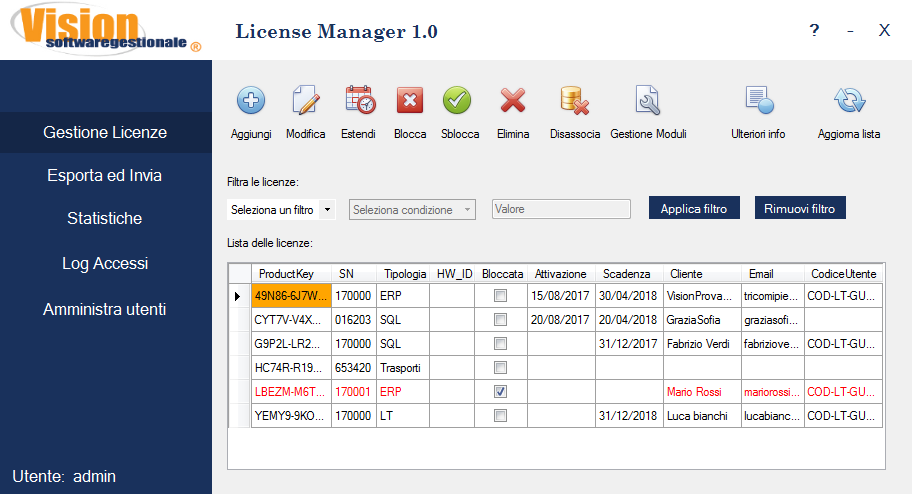
\includegraphics[width=0.9\columnwidth]{LicenseManager/gestLic} 
    \caption{License Manager 1.0 - Gestione Licenze.}
\label{gestLic}
\end{figure}

Nella sezione “Gestione Licenze“ è possibile gestire tutti gli aspetti delle licenze.
Nello specifico le operazioni permesse, nell'ordine, sono:
\begin{itemize}
\item \textbf{Aggiungi:} permette di creare una nuova licenza;
\item \textbf{Modifica:} permette di modificare diversi aspetti di una licenza;
\item \textbf{Estendi:} permette di posticipare la data di scadenza;
\item \textbf{Blocca:} permette di bloccare una licenza;
\item \textbf{Sblocca:} permette di sbloccare una licenza;
\item \textbf{Elimina:} permette di eliminare una licenza;
\item \textbf{Disassocia:} permette di dissociare una licenza dalle proprie componenti Hardware;
\item \textbf{Gestione Moduli:} permette di gestire i moduli della licenza;
\item \textbf{Ulteriori Info:} fornisce ulteriori informazioni sulla licenza;
\item \textbf{Aggiorna lista:} permette di aggiornare la lista delle licenze;
\item \textbf{Applica filtro:} permette di filtrare le licenze in base a determinate condizioni;
\item \textbf{Rimuovi filtro:} rimuove il filtro precedentemente selezionato.
\end{itemize} 
Nella parte alta della schermata sono presenti le funzionalità, mentre nella parte bassa è mostrata la lista delle licenze visibili all’utente.
\\
Un \textit{Admin} può visualizzare tutte le licenze, ed eventualmente filtrarle per \texttt{Codice Utente} per visualizzare le licenze assegnate a un rivenditore.
\\
Un \textit{Guest} (o rivenditore) può visualizzare solo le licenze con \texttt{Codice Utente} uguale al proprio.
\\

In generale, prima che avvenga una modifica a una licenza (o l'eliminazione), tramite l'utilizzo del Web Service \texttt{LicenseManagerService}, è salvato il suo stato attuale nella tabella \texttt{StoricoStatiLicenze} per avere lo storico completo di tutte le licenze. Inoltre, se la modifica è stata apportata da un \textit{Guest}, essa è notificata all'azienda tramite l'utilizzo del Web Service \textit{LicenseEmailService} per mantenere l'azienda informata sullo stato di tutte le licenze. 
\\Nei paragrafi successivi sono mostrate nel dettaglio tutte le funzionalità. 

\subsection{Aggiungi}
La funzione “Aggiungi” permette di creare una nuova licenza. Il metodo di creazione differisce per gli utenti Admin e gli utenti Guest. Cliccando sul pulsante si apre una nuova finestra, dove è possibile inserire i dati di una licenza. La finestra è riportata nella Figura \ref{crealic}.

\begin{figure}[!h] 
    \centering 
    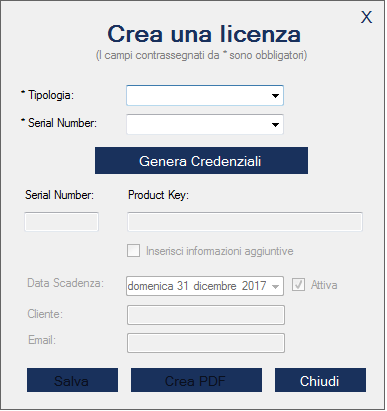
\includegraphics[width=0.55\columnwidth]{LicenseManager/creaLicenza} 
    \caption{Finestra Aggiungi - Gestione Licenze.}
    \label{crealic}
\end{figure}

Per creare una licenza è necessario innanzitutto valorizzare i campi obbligatori, ovvero \texttt{Tipologia} e \texttt{Serial Number}. 
\begin{itemize}

\item \textbf{Tipologia:} identifica quale licenza si sta creando, e i valori possibili sono SQL, LT, ERP o Trasporti; 
\item \textbf{Serial Number:} numero di sei cifre che identifica in modo univoco, per tipologia, una licenza. Uno stesso \texttt{Serial Number} è permesso per diverse tipologie. La scelta del \texttt{Serial Number} differisce da \textit{Admin} e \textit{Guest}.  
\begin{itemize}

\item	\textbf{Admin:} Può scegliere tra un \texttt{Serial Number}:
\begin{itemize}
\item \textbf{Manuale:} scelto arbitrariamente;
\item \textbf{Casuale:} generato casualmente dal programma;
\item \textbf{Prime due cifre per l'anno:} le prime due cifre sono le ultime due cifre dell'anno corrente, mentre le restanti quattro identificano il punto di partenza da cui cercare un \texttt{Serial Number} libero.
\end{itemize}
\item	\textbf{Guest:} Può creare solo un \texttt{Serial Number} di tipologia “Prime due cifre per l’anno”.
\end{itemize}

\end{itemize}	

Dopo aver scelto \texttt{Tipologia} e \texttt{Serial Number} è necessario cliccare su "Genera Credenziali" per continuare con la creazione della licenza. Cliccando su questo pulsante è invocato un metodo del Web Service \texttt{LicenseManagerService} che produrrà un \texttt{Serial Number} compatibile con la scelta effettuata e un \texttt{Product Key} che identifica univocamente una licenza, indipendentemente dalla tipologia. Qualora il \texttt{Serial Number} scelto in caso di selezione "Manuale" o "Casuale" fosse già in uso, sarà comunicato che non è possibile utilizzare tali valori ed è necessario sceglierne degli altri. In caso di scelta "Prime due cifre per l’anno" il \texttt{Serial Number} prodotto sarà il primo libero disponibile a partire dal numero a quattro cifre scelto. Dopo la creazione delle credenziali il pulsante "Salva" si attiverà e sarà possibile salvare la licenza, come si evince dalla Figura \ref{salva}.

 \begin{figure}[!h] 
    \centering 
    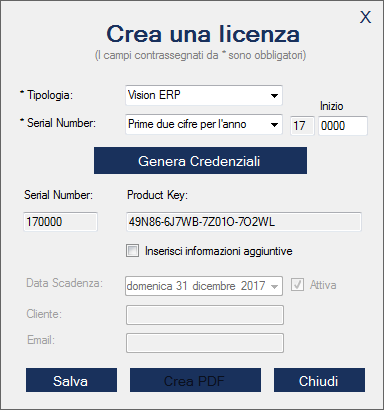
\includegraphics[width=0.55\columnwidth]{LicenseManager/salva} 
    \caption{License Manager 1.0 - Salvataggio di una licenza appena creata.}
\label{salva}
\end{figure}

Prima di procedere con il salvataggio è possibile definire delle informazioni aggiuntive della licenza, come la data di scadenza, il cliente cui è destinata e l’email da associare alla licenza. La data di scadenza può essere attivata o disattivata grazie alla checkbox "Attiva" a lato del selettore della data. Nel caso di inserimento di informazioni aggiuntive è possibile anche creare direttamente il PDF contenente i dettagli della licenza da spedire al cliente. Cliccando su "Crea PDF" sarà prima chiesto di salvare la licenza.
\\Nella Figura \ref{pdf} è mostrato l'inserimento delle informazioni aggiuntive con la creazione diretta del file PDF.


\begin{figure}[!h] 
    \centering 
    \includegraphics[width=0.9\columnwidth]{LicenseManager/creaPDFInfoAggi} 
    \caption{License Manager 1.0 - Informazioni aggiuntive e creazione file PDF.}
\label{pdf}
\end{figure}

Una licenza creata da un \textit{Guest} avrà come \texttt{Codice Utente} il suo codice, mentre se è creata da un \textit{Admin} esso sarà inizialmente nullo e potrà essere impostato in seguito attraverso la funzione "Modifica".
\\
L’esecuzione del salvataggio cambia a seconda di una creazione da parte di un \textit{Admin} o di un \textit{Guest}.
Solo se a creare la licenza è stato un \textit{Guest} viene prima notificata via mail l'azienda \textit{VISIONEIMPRESA s.r.l.}, attraverso l'utilizzo del Web Service \texttt{LicenseEmailService}, e poi si procede al salvataggio della licenza tramite l'utilizzo del Web Service \texttt{LicenseManagerService}. Se la notifica dovesse fallire l’operazione di salvataggio non viene eseguita, in quanto potrebbe sfuggire la creazione di una licenza. Se un errore dovesse incorrere durante il salvataggio sarà inviata una seconda mail per avvertire che la mail di creazione inviata in precedenza potrebbe essere errata.\\
Se a creare la licenza è un \textit{Admin} l'azienda non viene notificata.
\\
Infine, se la creazione è andata a buon fine, è mostrato un messaggio che lo conferma e la schermata di creazione viene chiusa. Nella lista delle licenze apparirà quindi la nuova licenza appena creata, come si può vedere nella Figura \ref{nuova}.

\begin{figure}[!h] 
    \centering 
    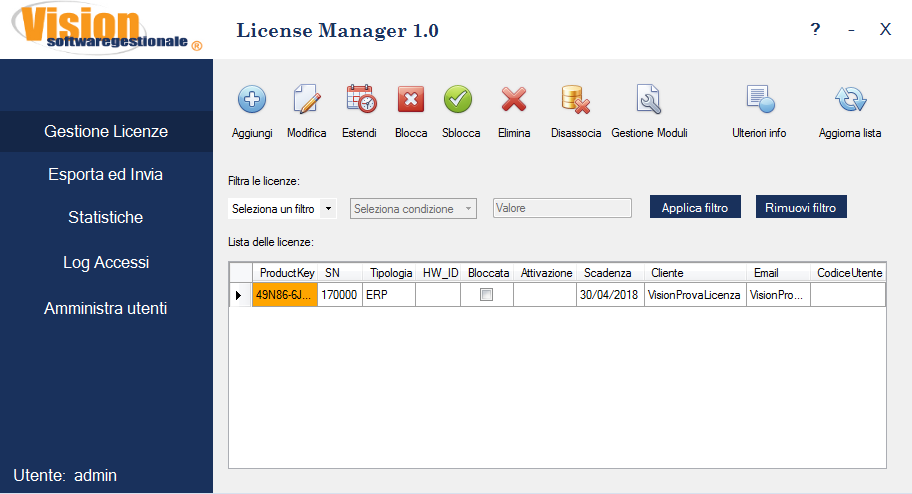
\includegraphics[width=0.85\columnwidth]{LicenseManager/nuovalicenza} 
    \caption{License Manager 1.0 - Aggiunta alla lista di una licenza appena creata.}
\label{nuova}
\end{figure}


\subsection{Modifica}

La funzione "Modifica" permette di modificare i dati non immutabili di una licenza:
\begin{itemize}
\item \textbf{Data di scadenza:} data di scadenza di una licenza, può anche essere rimossa;
\item \textbf{Cliente:} nome del cliente, utilizzato per comodità per riferirsi a una licenza;
\item \textbf{Email:} indirizzo email associato alla licenza. Tramite l’indirizzo email il cliente può disattivare e riattivare la propria licenza senza che sia necessario contattare l’azienda. Per questo motivo ai \textit{Guest} non è data la possibilità di modificare l’email decisa dai clienti in fase di attivazione;
\item \textbf{Codice Utente:} codice del rifornitore cui è assegnata la licenza. Un rifornitore sarà in grado di vedere solo le licenze con il \texttt{Codice Utente} uguale a quello a lui assegnato. Per questo motivo anche il \texttt{Codice Utente} non può essere modificato dai rifornitori.
Gli \textit{Admin}, invece, possono vedere tutte le licenze e modificarne il \texttt{Codice Utente}, a meno che la licenza non sia impostata come "Licenza ad uso interno non rivendibile". Riferirsi alla sezione \ref{gestmod} per ulteriori informazioni.
\end{itemize} 

In Figura \ref{modifica} è mostrata la schermata di modifica.

\begin{figure}[!h] 
    \centering 
    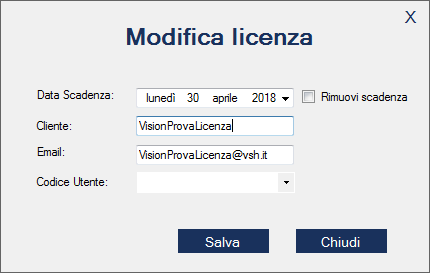
\includegraphics[width=0.6\columnwidth]{LicenseManager/modifica} 
    \caption{License Manager 1.0 - Modifica di una licenza.}
\label{modifica}
\end{figure}

\newpage
\subsection{Estendi}
La funzione "Estendi" permette di modificare velocemente la data di scadenza, scegliendone una nuova o indicando il numero di mesi di cui si vuole estendere la licenza.
Il Form relativo è mostrato in Figura \ref{estendi}.

\begin{figure}[!h] 
    \centering 
    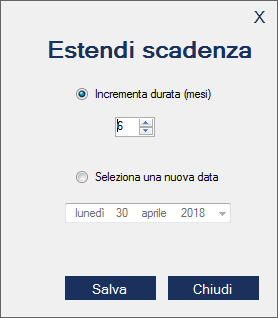
\includegraphics[width=0.45\columnwidth]{LicenseManager/Estendi} 
    \caption{License Manager 1.0 - Estensione del periodo di validità di una licenza.}
\label{estendi}
\end{figure}

\subsection{Blocca}

La funzione "Blocca" permette di bloccare una licenza. All’accesso del \textit{Software Gestionale Vision} se la licenza è bloccata viene mostrato un messaggio d’errore e non è permesso l’utilizzo.
Le licenze bloccate sono mostrate in rosso nella lista delle licenze, cosi come le licenze scadute.
È possibile anche bloccare più licenze in una volta selezionandole dalla lista.
\\
Nella Figura \ref{block} si può vedere un esempio di licenza bloccata.
\begin{figure}[!h] 
    \centering 
    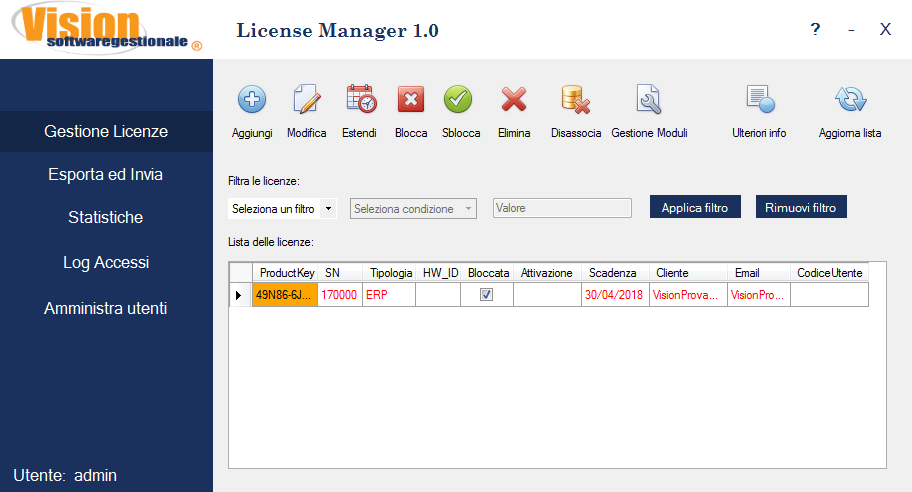
\includegraphics[width=0.8\columnwidth]{LicenseManager/bloccate} 
    \caption{License Manager 1.0 - Licenza bloccata.}
\label{block}
\end{figure}

\subsection{Sblocca}
La funzione "Sblocca" permette di sbloccare una licenza bloccata in precedenza.
I rivenditori possono sbloccare solo le licenze da loro bloccate, per evitare di rimuovere i blocchi imposti dagli \textit{Admin}.\\
Come si vede nella Figura \ref{sblocca}, accedendo con un utente di tipo \textit{Guest} (in questo caso "ProvaLT"), non è possibile sbloccare una licenza bloccata da un \textit{Admin}.

\begin{figure}[!h] 
    \centering 
    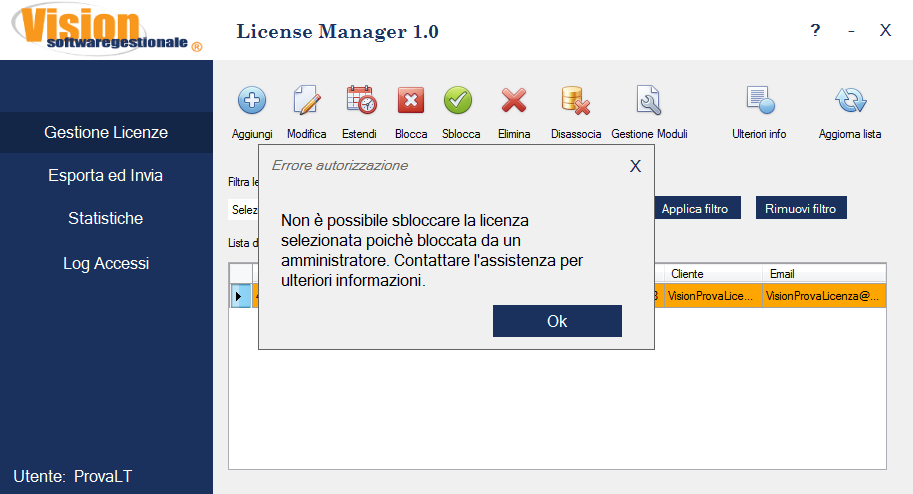
\includegraphics[width=0.8\columnwidth]{LicenseManager/sblocca} 
    \caption{License Manager 1.0 - Sblocco di una licenza.}
\label{sblocca}
\end{figure}

\subsection{Elimina}
La funzione “Elimina” permette di rimuovere una licenza, tuttavia agisce in modo diverso se a richiedere l'eliminazione è un \textit{Admin} o un \textit{Guest}. Mentre per l’\textit{Admin} l’eliminazione è sempre concessa, un \textit{Guest} può eliminare la licenza solo se non è mai stata attivata o se non sono ancora stati definiti i moduli per quella licenza.\\
Nella Figura \ref{elim} l’utente \textit{Guest} "ProvaLT", tentando l’eliminazione dopo che i moduli della licenza sono stati definiti, viene avvisato e l’eliminazione non avviene.

\begin{figure}[!h] 
    \centering 
    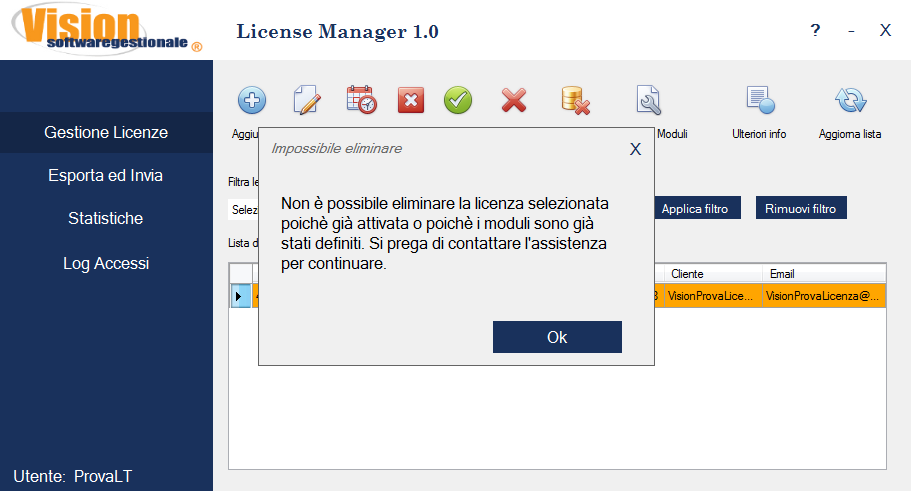
\includegraphics[width=0.8\columnwidth]{LicenseManager/elimin} 
    \caption{License Manager 1.0 - Eliminazione di una licenza.}
\label{elim}
\end{figure}

\subsection{Disassocia}

La funzione "Disassocia" permette di dissociare una licenza dalle sue componenti Hardware, utilizzate per verificare che la licenza sia in uso su un solo computer per volta. 
Dissociando una licenza dalle sue componenti Hardware se ne permette la reinstallazione in una nuova macchina, mentre su quella attuale all’avvio del \textit{Software Gestionale Vision} risulterà che la licenza non è più associata a quel dispositivo.

\subsection{Gestione Moduli}
\label{gestmod}
La funzione "Gestione Moduli" permette di selezionare quali moduli associare a una licenza. Sia \textit{Admin} che \textit{Guest} possono selezionare i moduli, ma con delle differenze: gli \textit{Admin} possono modificare i moduli un qualsiasi numero di volte, mentre i \textit{Guest} possono impostarli solo una volta dopo la creazione, dopodiché la modifica non sarà più permessa. Se i moduli sono già stati definiti da un \textit{Admin} allora il \textit{Guest} non potrà modificarli.
Cliccando su "Gestione Moduli", in base alla tipologia della licenza, si apre una nuova finestra che si presenta come nella Figura \ref{gest}.

\begin{figure}[!h] 
    \centering 
    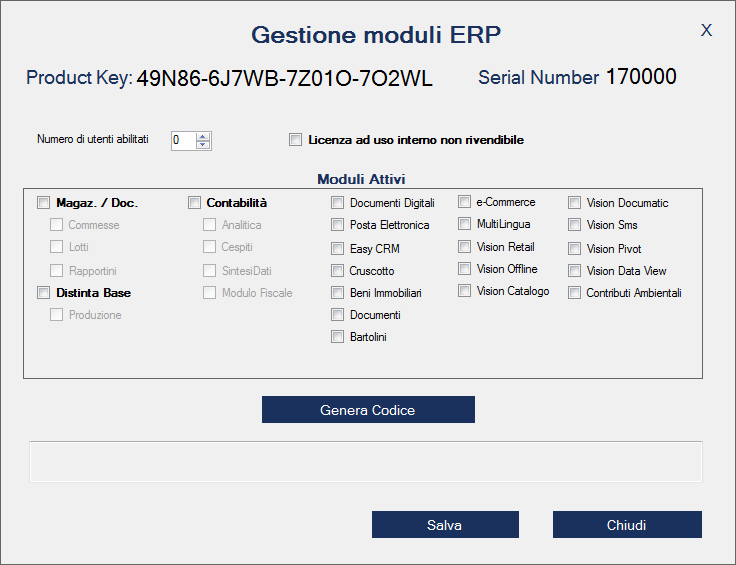
\includegraphics[width=1\columnwidth]{LicenseManager/gestmoduli} 
    \caption{License Manager 1.0 - Gestione dei moduli di una licenza.}
\label{gest}
\end{figure}

Da qui è possibile selezionare il numero di utenti abilitati e i moduli da attivare. Inoltre a un \textit{Admin} è permesso impostare la licenza come "Licenza ad uso interno non rivendibile", che selezionerà automaticamente tutti i moduli e non potrà essere associata a un codice utente.\\
Una volta scelti i moduli è necessario cliccare su "Genera Codice" per generare il codice riassuntivo dei moduli scelti, che viene creato come dal programma \textit{GenFileKey}. Il codice generato è quindi il codice cifrato che in precedenza veniva salvato nei file di configurazione ".HWK".  Dopo aver generato il codice, la situazione si presenta come nella Figura \ref{codcreat}.

\begin{figure}[!h] 
    \centering 
    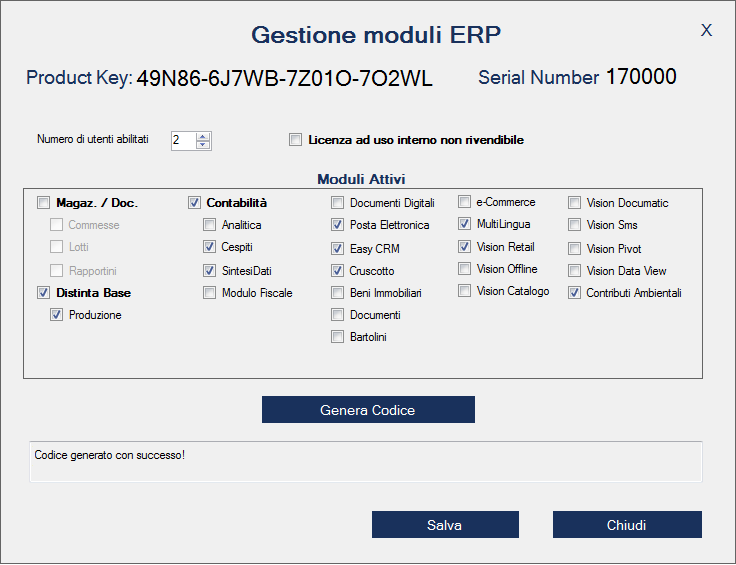
\includegraphics[width=1\columnwidth]{LicenseManager/codgen} 
    \caption{License Manager 1.0 - Creazione del codice moduli.}
\label{codcreat}
\end{figure}

Nel caso a generare il codice fosse un \textit{Admin}, nel riquadro al posto di "Codice generato con successo!" sarebbe mostrato il codice generato.
\\
A questo punto è necessario salvare con il pulsante "Salva" per rendere effettive le modifiche.
Un \textit{Admin} può definire più volte i moduli nella stessa schermata, ma dopo aver salvato la prima volta è necessario rigenerare il codice per poter salvare nuovamente.\\
L’esecuzione del salvataggio cambia a seconda della definizione dei moduli da parte di un \textit{Admin} o di un \textit{Guest}.
Solo se a creare la licenza è stato un \textit{Guest} viene prima notificata via mail l'azienda \textit{VISIONEIMPRESA s.r.l.}, attraverso l'utilizzo del Web Service \texttt{LicenseEmailService}, e poi si procede al salvataggio dei moduli tramite l'utilizzo del Web Service \texttt{LicenseManagerService}. Se la notifica dovesse fallire l’operazione di salvataggio non viene eseguita, in quanto potrebbe sfuggire la definizione dei moduli, operazione fondamentale per una corretta fatturazione della licenza. Se un errore dovesse incorrere durante il salvataggio sarà inviata una seconda mail per avvertire che la mail inviata in precedenza potrebbe essere errata.
Una mail riepilogativa dei moduli è inviata anche all'indirizzo email associato all'utente che sta definendo i moduli.

\newpage

\subsection{Ulteriori Info}
La funzione "Ulteriori Info" permette di visualizzare delle informazioni aggiuntive sulla lista, non visibili nella lista delle licenze.
La schermata mostrata è visibile nella Figura \ref{info}.


\begin{figure}[!h] 
    \centering 
    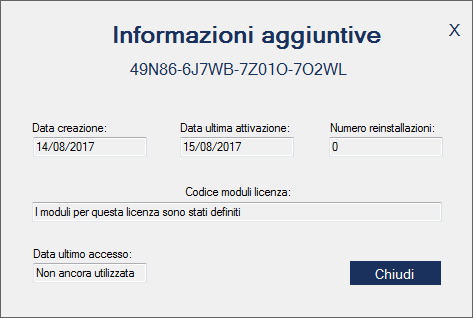
\includegraphics[width=0.7\columnwidth]{LicenseManager/ultInfo} 
    \caption{License Manager 1.0 - Creazione del codice moduli.}
\label{info}
\end{figure}

Le informazioni fornite sono:

\begin{itemize}
\item \textbf{Data creazione:} data di creazione della licenza;
\item \textbf{Data ultima attivazione:} data in cui la licenza è stata attivata l’ultima volta, poiché un utente finale può disattivare e attivare una propria licenza senza limiti;
\item \textbf{Numero reinstallazioni:} quante reinstallazioni sono state eseguite dall’utente;
\item \textbf{Codice moduli licenza:} codice riepilogativo dei moduli selezionati se chi visualizza è un \textit{Admin}, altrimenti è mostrato se i moduli sono stati definiti o meno; 
\item \textbf{Data ultimo accesso:} data ultima in cui l’utente ha usato il \textit{Software Gestionale Vision} legato a quella licenza.

\end{itemize}

\subsection{Aggiorna Lista}
La funzione "Aggiorna lista" permette di ricaricare la lista delle licenze. Nel riaggiornare, è chiesto se si vogliono mantenere i filtri di ricerca eventualmente impostati in precedenza.

\subsection{Applica Filtro}
La funzione "Applica filtro" permette di applicare dei filtri sui campi delle licenze. Tra i filtri disponibili agli \textit{Admin} è selezionabile "Codice Utente", che permette di quindi di restringere il campo delle licenze visibili a quelle di un solo utente, per monitorare le licenze di un rivenditore.\\
Un filtro, in generale, è formato da tre parametri: il campo da filtrare (ad esempio \texttt{Product Key} o \texttt{Serial Number}), la condizione da applicare (ad esempio "Uguale" o "Contiene") e il valore con cui applicare il filtro.

\subsection{Rimuovi Filtro}
La funzione "Rimuovi filtro" rimuove il filtro selezionato in precedenza, tornando a mostrare tutte le licenze visibili all’utente.


%**************************************************************

\section{Esporta ed Invia}

Nella sezione "Esporta ed Invia" è possibile esportare alcuni dati relativi alle licenze o creare un documento riepilogativo della licenza selezionata. Come per la sezione "Gestione Licenze" saranno mostrate solo le licenze compatibili con il \texttt{Codice Utente} dell’utente che ha effettuato l'accesso. I campi qui mostrati riguardano i contatti delle licenze.
In Figura \ref{espinv} è possibile vedere una situazione esempio della sezione.

\begin{figure}[!h] 
    \centering 
    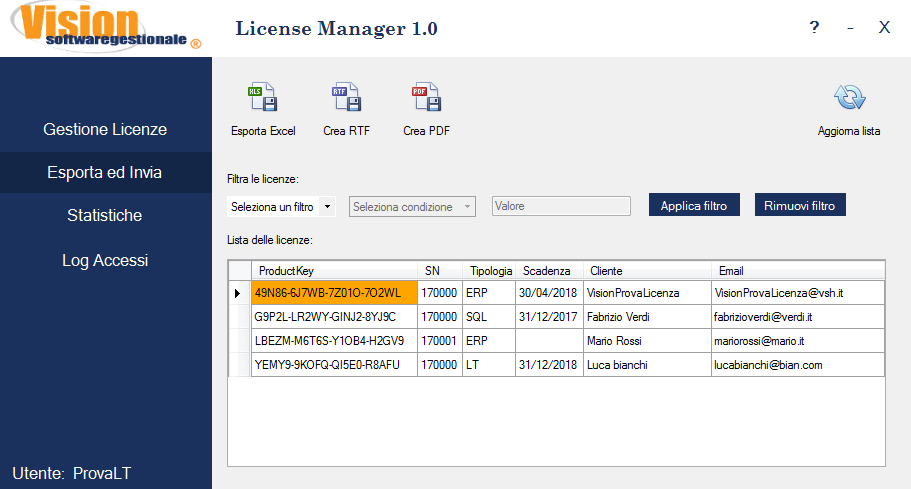
\includegraphics[width=0.9\columnwidth]{LicenseManager/esportainvia} 
    \caption{License Manager 1.0 - Sezione Esporta ed Invia.}
\label{espinv}
\end{figure}

Nei paragrafi successivi sono mostrate nel dettaglio tutte le funzionalità. 

\subsection{Esporta Excel}

La funzione "Esporta Excel" permette di esportare in un file ".xls" due tipologie di dati:
\begin{itemize}

\item \textbf{Tutti i dati:} esporta tutte le licenze visibili all’utente con tutti i loro dati. Nel caso a esportare i dati fosse un \textit{Guest} non sarebbe mostrato il \texttt{Codice Moduli} e il \texttt{Codice Utente} per motivi di sicurezza.
\item \textbf{Contatti:} esporta solo i contatti riguardanti le licenze, ovvero tutti i campi visibili in questa schermata.

\end{itemize}

L'ottenimento dei dati avviene tramite il Web Service \texttt{LicenseManagerService}.

\subsection{Crea RTF}
\label{creartf}
La funzione "Crea RTF" permette di creare un file RTF contenente il riepilogo della licenza da inviare al cliente al momento dell’acquisto. La creazione del file avviene secondo un file modello posto nella cartella di installazione di \textit{License Manager 1.0}. Se questo modello non è presente viene utilizzato un modello standard.

Il file modello è simile a quello mostrato in Figura \ref{modello}.

\begin{figure}[!h] 
    \centering 
    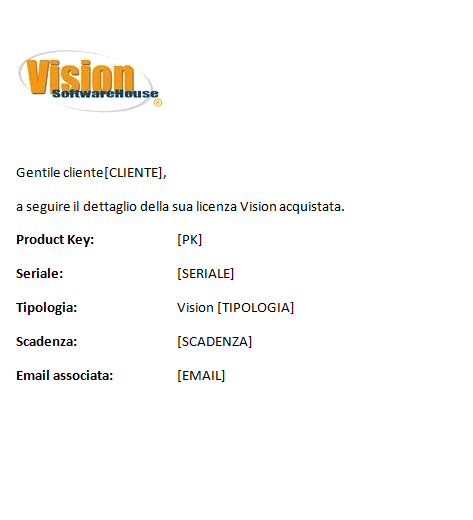
\includegraphics[width=0.7\columnwidth]{LicenseManager/modello} 
    \caption{Modello riepilogativo di una licenza.}
\label{modello}

\end{figure}

Il programma sostituisce i parametri contenuti tra parentesi quadre e genera il file finale. Qualora si voglia utilizzare un nuovo modello, è sufficiente collocare le scritte tra parentesi quadre nella posizione desiderata all’interno del file e il programma provvederà a sostituirle con i valori opportuni.

\subsection{Crea PDF}

La funzione "Crea PDF" permette di creare un file PDF partendo dal modello RTF disponibile, o in caso di assenza secondo un modello standard, come spiegato nella sezione \ref{creartf}.

\subsection{Aggiorna Lista}
La funzione "Aggiorna lista" permette di ricaricare la lista delle licenze. Nel riaggiornare, è chiesto se si vogliono mantenere i filtri di ricerca eventualmente impostati in precedenza.

\subsection{Applica Filtro}
La funzione "Applica filtro" permette di applicare dei filtri sui campi delle licenze. Tra i filtri disponibili agli \textit{Admin} è selezionabile "Codice Utente", che permette di quindi di restringere il campo delle licenze visibili a quelle di un solo utente, per monitorare le licenze di un rivenditore.

\subsection{Rimuovi Filtro}
La funzione "Rimuovi filtro" rimuove il filtro selezionato in precedenza, tornando a mostrare tutte le licenze visibili all’utente.


%**************************************************************
\section{Statistiche}

Nella sezione "Statistiche" è possibile avere un quadro riassuntivo delle proprie licenze, o nel caso di un \textit{Admin} di tutte le licenze o di quelle del rivenditore selezionato.\\
In Figura \ref{stat} è possibile vedere una situazione esempio della sezione.


\begin{figure}[!h] 
    \centering 
    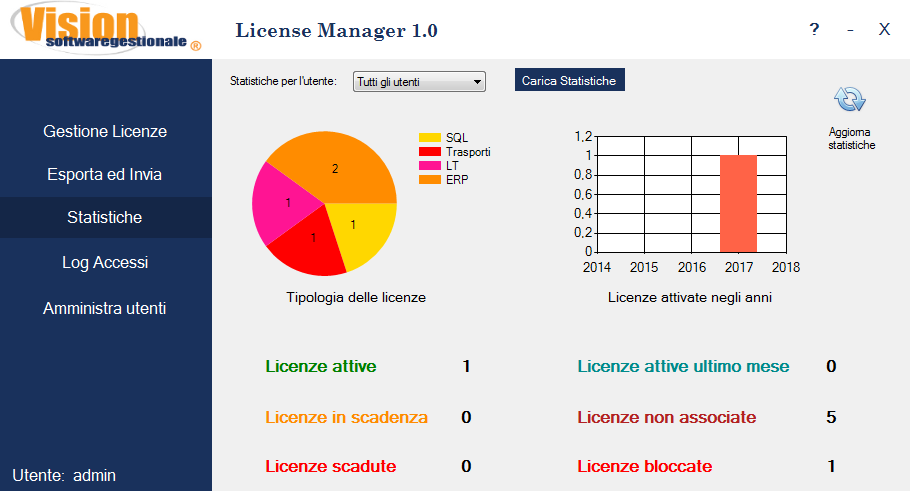
\includegraphics[width=0.9\columnwidth]{LicenseManager/statistiche} 
    \caption{License Manager 1.0 - Sezione Statistiche.}
\label{stat}

\end{figure}

Attraverso la combobox "Statistiche per l’utente" (visibile ai soli \textit{Admin}) si può scegliere per quale rivenditore visualizzare le statistiche. Selezionando "Tutti gli utenti" si avranno le statistiche su tutte le licenze. È necessario cliccare su "Carica Statistiche" per applicare il filtro dell’Utente.\\
Le statistiche mostrate sono le seguenti:

\begin{itemize}

\item \textbf{Tipologia delle licenze:} grafico a torta che mostra il numero di licenze per tipologia;
\item \textbf{Licenze attivate negli anni:} grafico a barre che mostra il numero di licenze attivate per ognuno degli ultimi tre anni;
\item \textbf{Licenze attive:} quante licenze sono state attivate;
\item \textbf{Licenze in scadenza:} quante licenze scadranno nei prossimi tre mesi;
\item \textbf{Licenze scadute:} quante licenze sono scadute;
\item \textbf{Licenze attive ultimo mese:} quante licenze sono state usate nell’ultimo mese attraverso il \textit{Software Gestionale Vision};
\item \textbf{Licenze non associate:} quante licenze non hanno componenti Hardware associate;
\item \textbf{Licenze bloccate:} quante licenze sono bloccate.

\end{itemize}

L'ottenimento dei dati avviene tramite il Web Service \texttt{LicenseManagerService}.

%**************************************************************
\section{Log Accessi}

Nella sezione "Log Accessi" è possibile monitorare gli accessi al \textit{Software Gestionale Vision}, legando al \texttt{Product Key} utilizzato per l’attivazione l’\texttt{indirizzo IP} e il \texttt{MAC Address} della scheda di rete utilizzati per connettersi a Internet. In questo modo è possibile venire a conoscenze di alcune anomalie come accessi multipli da diverse postazioni, qualora i controlli fossero stati evasi.\\
In Figura \ref{accessi} è possibile vedere una situazione esempio della sezione.
\begin{figure}[!h] 
    \centering 
    \includegraphics[width=0.9\columnwidth]{LicenseManager/logAccessi} 
    \caption{License Manager 1.0 - Sezione Log Accessi.}
\label{accessi}

\end{figure}

\subsection{Funzionalità}

Sotto le voci "Licenze con multipli IP" e "Licenze con multipli MAC Address" sono mostrate quante licenze hanno rispettivamente più di un \texttt{indirizzo IP} e più {MAC Address} associati.
Se una licenza dovesse avere più di due indirizzi associati verrebbe contata comunque una sola volta.\\
Cliccando su "Licenze con multipli IP" vengono selezionati in verde il \texttt{Product Key} e \texttt{l’indirizzo IP} dei record che hanno un \texttt{indirizzo IP} diverso dalla prima occorrenza per quel \texttt{Product Key}.\\
Cliccando su "Licenze con multipli MAC Address" vengono selezionati in rosso il \texttt{Product Key} e il \texttt{MAC Address} dei record che hanno un \texttt{MAC Address} diverso dalla prima occorrenza per quel \texttt{Product Key}.
In caso una licenza avesse sia diverso \texttt{indirizzo IP} sia diverso \texttt{MAC Address} il \texttt{Product Key} è evidenziato in viola.\\
Il funzionamento illustrato in precedenza è mostrato nella Figura \ref{multip}.

\begin{figure}[!h] 
    \centering 
    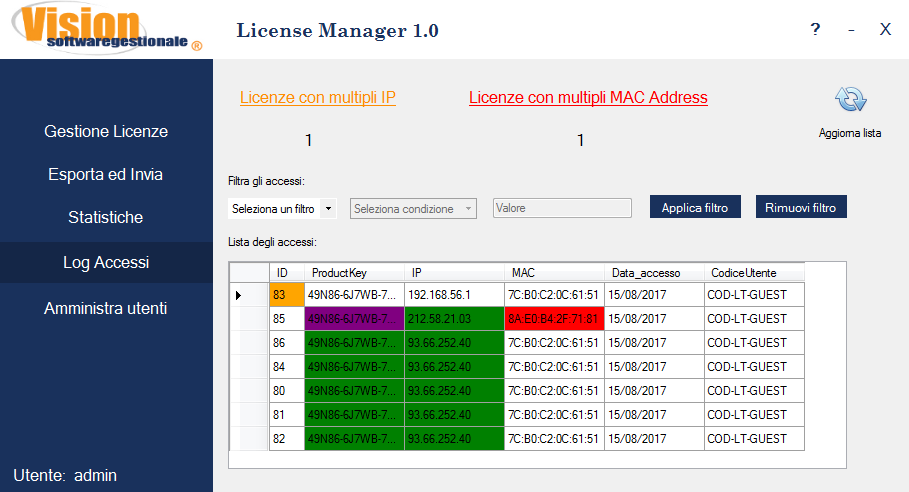
\includegraphics[width=0.9\columnwidth]{LicenseManager/multip} 
    \caption{License Manager 1.0 - Selezione delle licenze con multipli IP e MAC Address.}
\label{multip}

\end{figure}

Gli accessi al \textit{Software Gestionale Vision} sono ottenuti tramite l'utilizzo del Web Service \texttt{LicenseManagerService}.


%**************************************************************
\section{Amministra Utenti}
\label{ammut}
La sezione "Amministra utenti" è visibile ai soli utenti \textit{Admin} e permette di gestire gli utenti del programma \textit{License Manager 1.0}.\\
In Figura \ref{amm} è possibile vedere una situazione esempio della sezione.
\begin{figure}[!h] 
    \centering 
    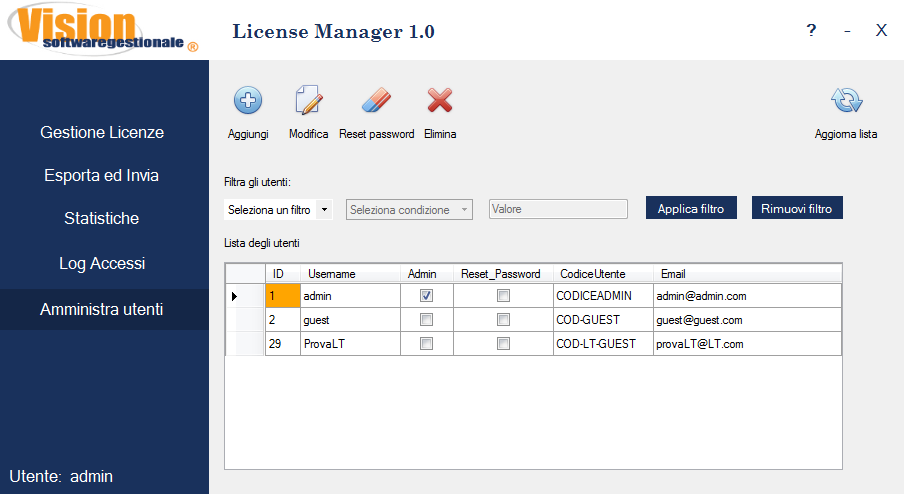
\includegraphics[width=0.9\columnwidth]{LicenseManager/amministra} 
    \caption{License Manager 1.0 - Sezione Amministra Utenti.}
\label{amm}

\end{figure}

Nella parte alta della schermata sono presenti le funzionalità, mentre nella parte bassa è mostrata la lista degli utenti con le loro caratteristiche.\\
Nello specifico le operazioni permesse, nell'ordine, sono:
\begin{itemize}
\item \textbf{Aggiungi:} permette di creare un nuovo utente;
\item \textbf{Modifica:} permette di modificare un utente;
\item \textbf{Reset password:} concede o rimuove la possibilità di un utente di resettare la propria password;
\item \textbf{Elimina:} permette di eliminare un utente.
\end{itemize}

Nei paragrafi successivi sono mostrate nel dettaglio tutte le funzionalità. 

\subsection{Aggiungi}


La funzione "Aggiungi" permette di creare un nuovo utente. La finestra che si presenta è mostrata in Figura \ref{agg}.

\begin{figure}[!h] 
    \centering 
    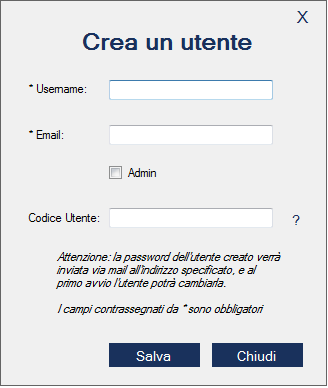
\includegraphics[width=0.4\columnwidth]{LicenseManager/aggut} 
    \caption{License Manager 1.0 - Creazione di un utente.}
\label{agg}

\end{figure}

I campi Username ed Email sono obbligatori.
\begin{itemize}
\item \textbf{Username:} identifica univocamente un utente, credenziale necessaria per l’accesso;
\item \textbf{Email:} lega un utente a una mail, che sarà utilizzata sia per l’invio della password da utilizzare per il primo accesso sia per le notifiche di creazione di nuove licenze da parte di un rivenditore.
\end{itemize}
Il campo \texttt{Admin}, se selezionato, identifica l’utente come \textit{Admin}, fornendone tutti i privilegi.\\
Il \texttt{Codice Utente} è deciso manualmente alla creazione o in seguito attraverso la funzione di modifica utente, e serve per identificare un utente con il proprio codice rivenditore. Più utenti possono avere lo stesso \texttt{Codice Utente}, e saranno quindi in grado di gestire le stesse licenze. Gli \textit{Admin} hanno il \texttt{Codice Utente} sempre impostato a "CODICEADMIN", il che li differenzia dagli altri utenti \textit{Guest}.\\
Dopo aver salvato l’utente, tramite l'utilizzo del Web Service \texttt{LicenseManagerService} è inviata una mail all’indirizzo scelto contenente l’username e la password da utilizzare per il primo accesso. Dopo l’accesso, è richiesto l’inserimento di una nuova password per questioni di sicurezza.


\subsection{Modifica}

La funzione "Modifica" permette di modificare un utente. La finestra che si presenta è mostrata in Figura \ref{mod}.

\begin{figure}[!h] 
    \centering 
    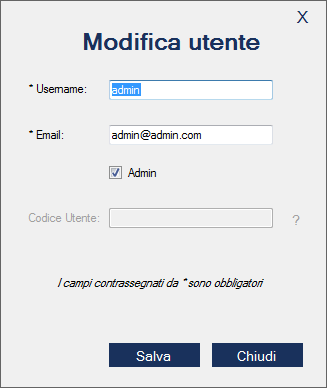
\includegraphics[width=0.4\columnwidth]{LicenseManager/modut} 
    \caption{License Manager 1.0 - Modifica di un utente.}
\label{mod}

\end{figure}

Con questo Form può essere modificato l’username, l'indirizzo email associato all’account e fornire o rimuovere i privilegi di \textit{Admin}. Qualora l’utente sia un \textit{Admin} non è possibile scegliere un \texttt{Codice Utente} poiché sarà impostato di default a "CODICEADMIN".

\subsection{Reset password}

La funzione "Reset password" permette all’utente selezionato di poter reimpostare la password alla prossima autenticazione. Il reset della password deve avvenire sempre tramite il permesso di un \textit{Admin}, e non sono previsti altri metodi.
\\
Per resettare la password qualora l’utente non ricordasse la vecchia, è sufficiente inserire l’\texttt{Username} nel campo apposito del Form di autenticazione e cliccare su "Password dimenticata?".\\
È possibile per un Admin resettare la propria password seguendo la stessa procedura, scegliendone una nuova al prossimo accesso.
\\
In Figura \ref{reset} è mostrato il processo di reset della password tramite il Form di autenticazione.

\begin{figure}[!h] 
    \centering 
    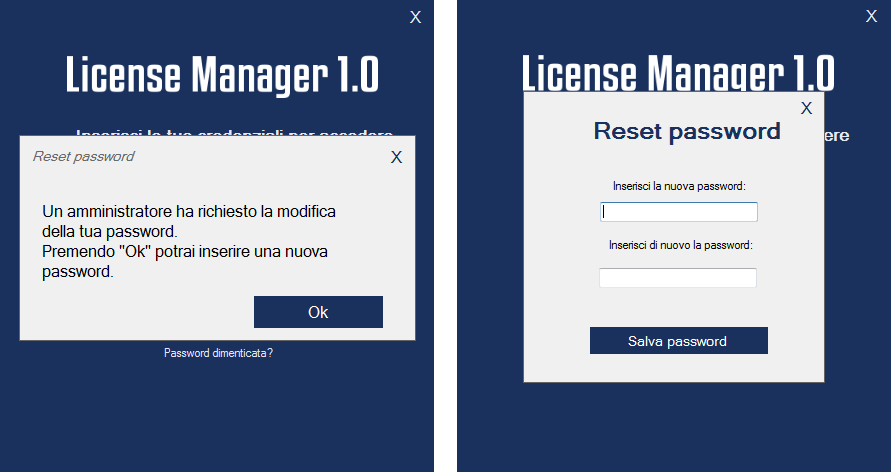
\includegraphics[width=1\columnwidth]{LicenseManager/reset} 
    \caption{License Manager 1.0 - Reset della password di un utente.}
\label{reset}

\end{figure}


\newpage
\subsection{Elimina}

La funzione "Elimina" permette di eliminare un utente di \textit{License Manager 1.0}, tranne se stessi. Per eliminare un \textit{Admin} è necessario svolgere l’operazione da un altro account \textit{Admin}. Poiché l’eliminazione è sempre permessa, si consiglia di limitare al minimo il numero di utenti \textit{Admin} presenti.